\documentclass[12pt,a4paper,oneside]{article}
\usepackage{amsmath,amsthm,amsfonts,amssymb}
\usepackage{pst-eucl,pstricks,pstricks-add}
\usepackage[utf8]{inputenc}
\usepackage{pgfkeys, pgfsys, pgfcalendar}
%\usepackage[latin1]{inputenc}
\usepackage[spanish,activeacute]{babel}
\usepackage[a4paper,margin=2.5cm]{geometry}
\usepackage{times}
\usepackage[T1]{fontenc}
\usepackage{titlesec}
\usepackage{color}
\usepackage{url}
\usepackage{float}
\usepackage{cite}
\usepackage{graphicx}
\usepackage{multicol}
\usepackage{lipsum}
\usepackage{transparent}
\usepackage{eso-pic}
%\AddToShipoutPic& re*{
   % \put(0,0){
        %\parbox[b][\paperheight]{\paperwidth}{$\$\%$$
           % \vfill
            %\centering
            %{\transparent{0.5}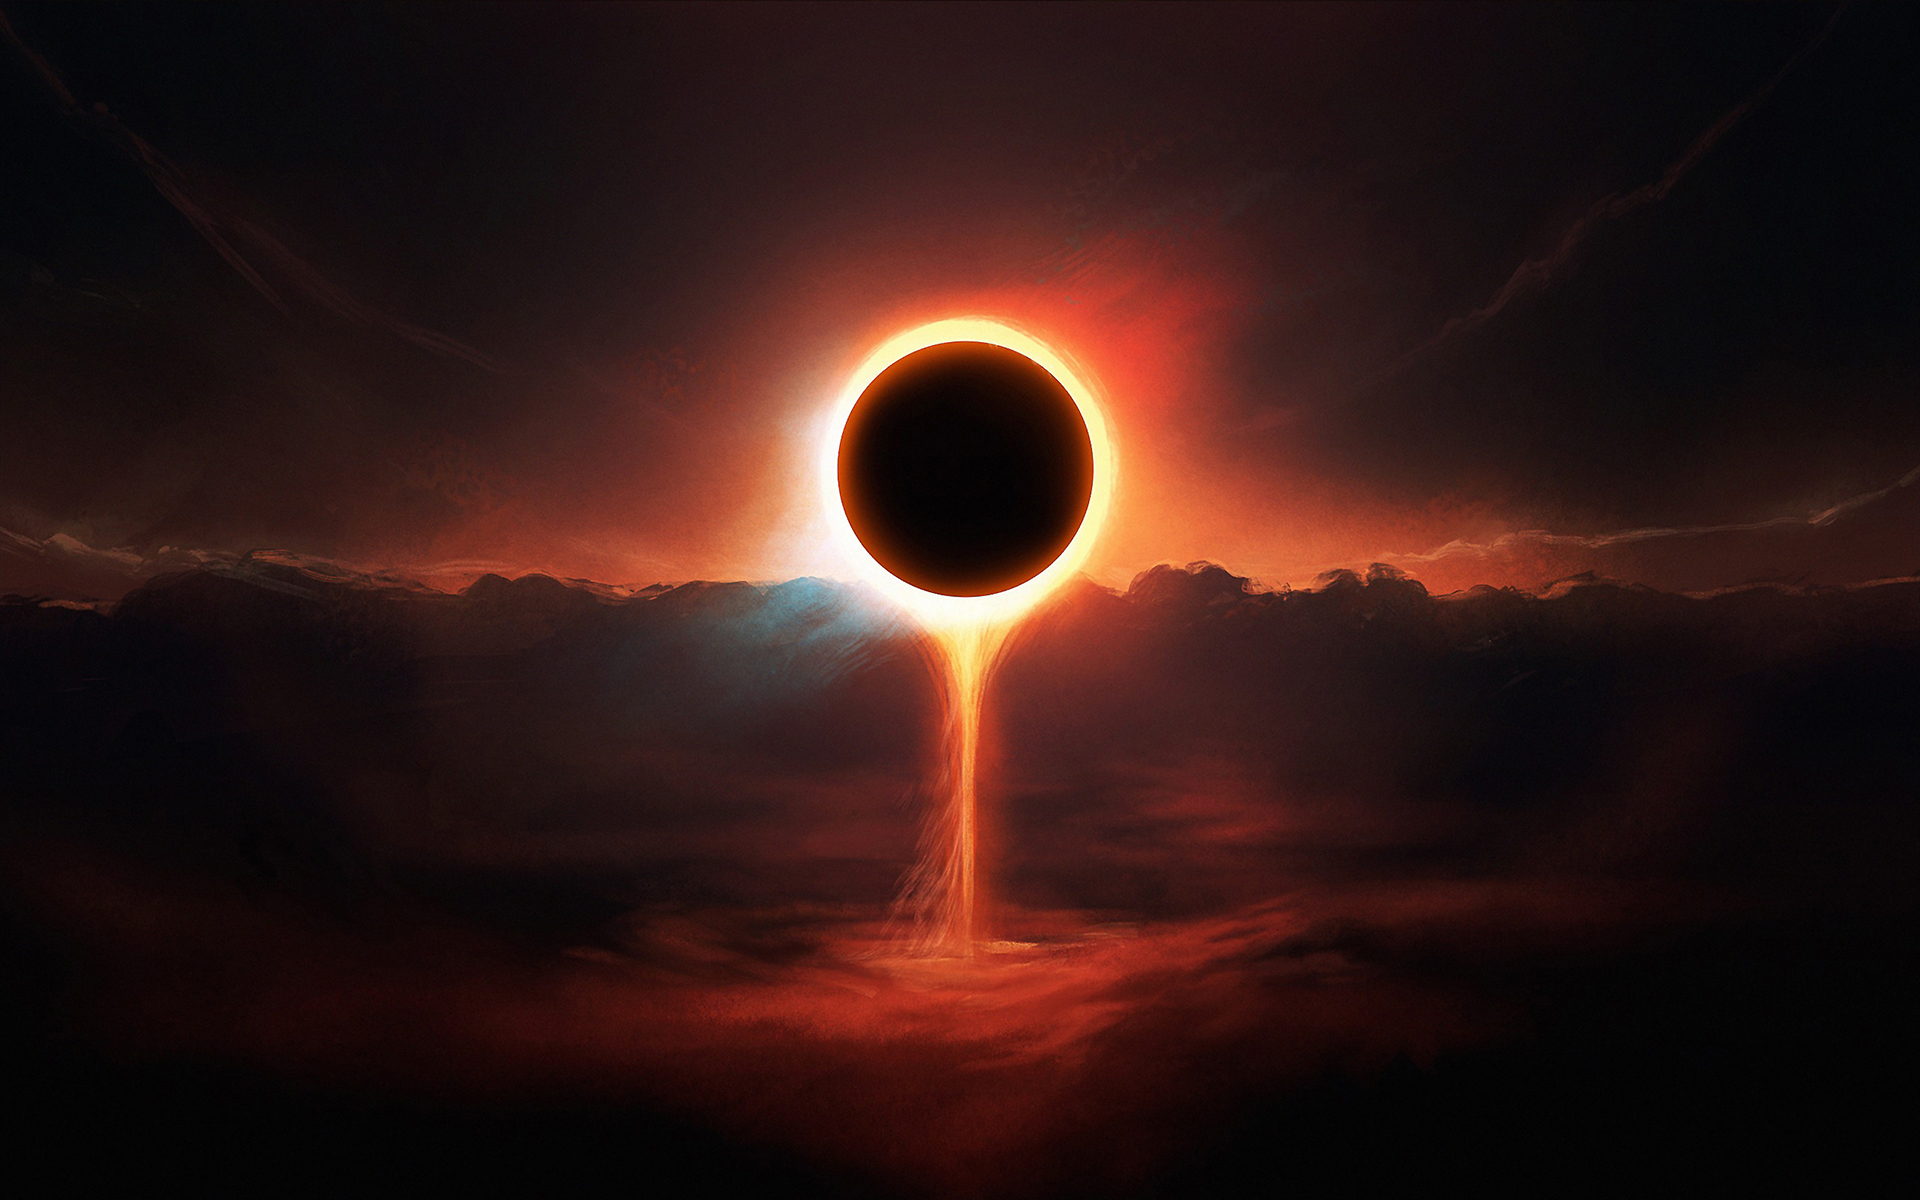
\includegraphics[width=3.5\textwidth]{febrero}}$\$\%$$
           % \vfill
       % }
   % }
%}
%\AddToShipoutPic& re*{
   % \put(0,0){
      %  \parbox[b][\paperheight]{\paperwidth}{$\$\%$$
           % \vfill
           % \centering
           % {\transparent{0.5}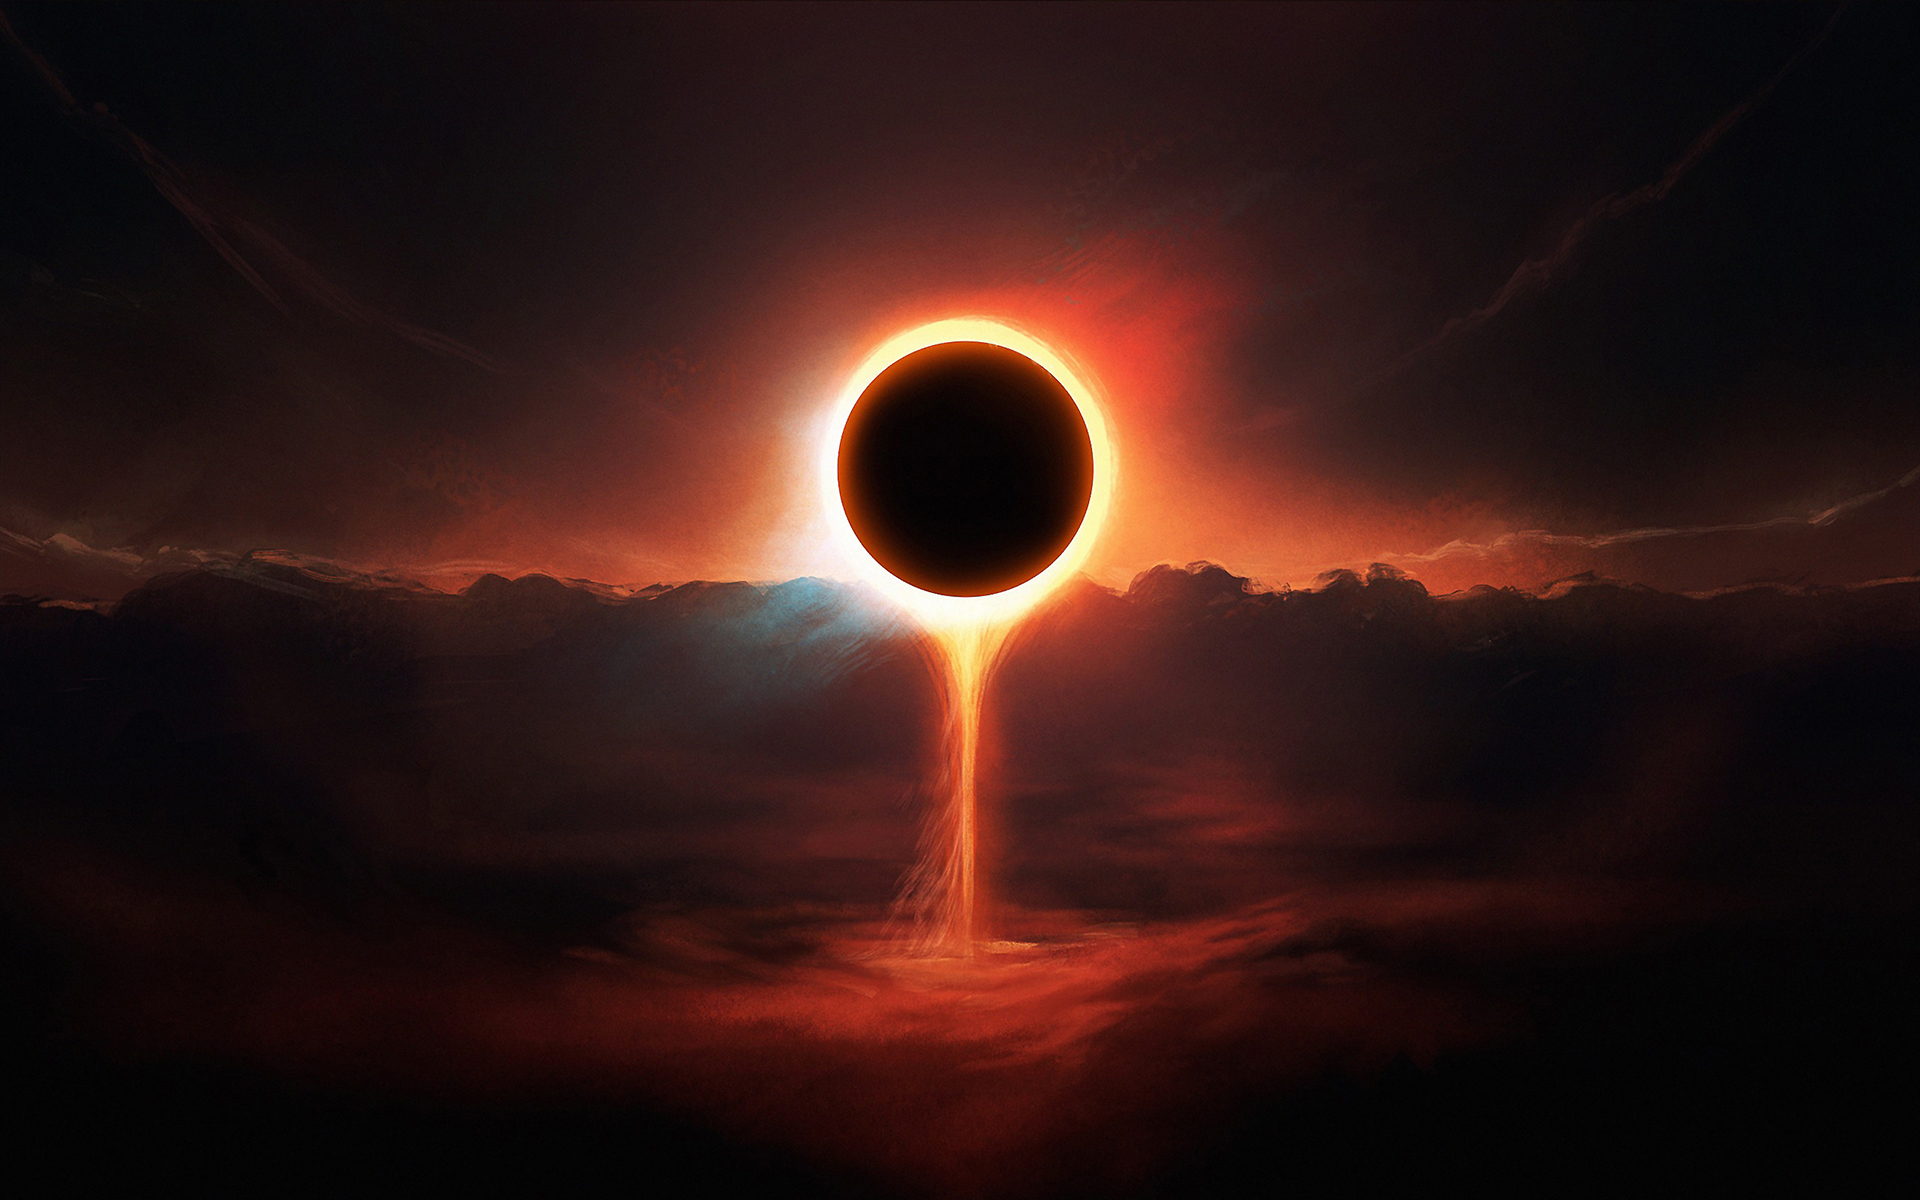
\includegraphics[width=3\textwidth]{febrero}}$\$\%$$
          %  \vfill
       % }
    %}
%}

%\usepackage{draftwatermark} %comente esta línea para obtener las efemérides sin fondo
%\SetWatermarkText{\transparent{0.4}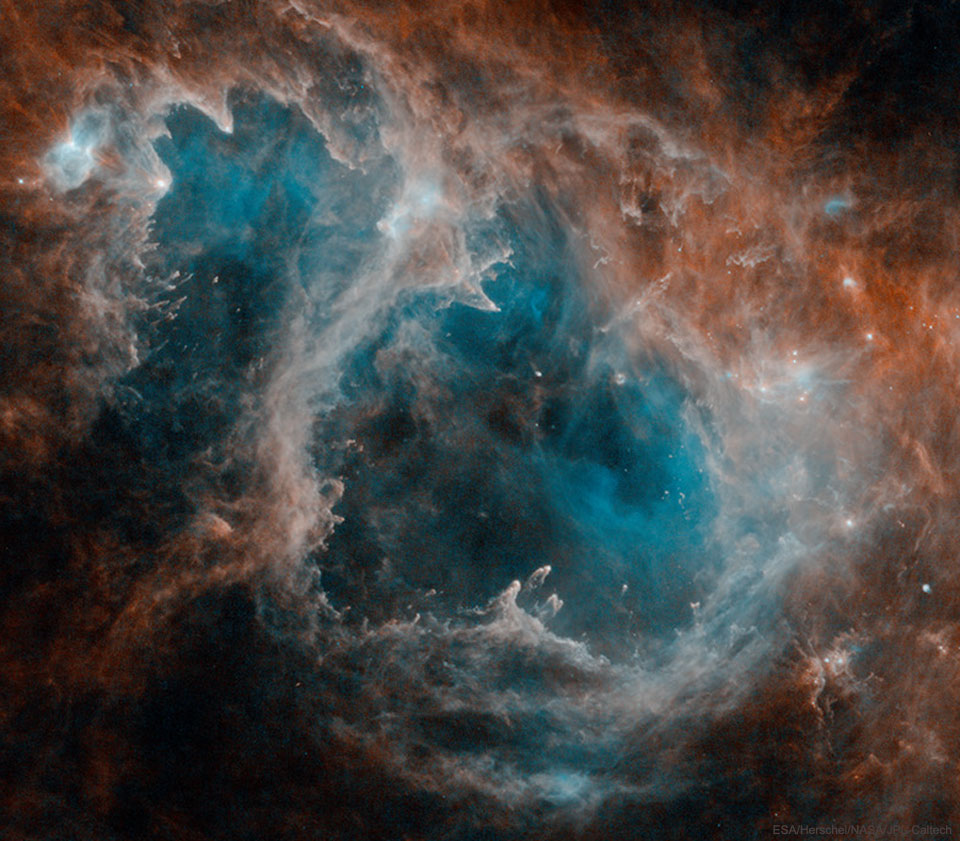
\includegraphics[scale=1,clip,angle=-135]{fondo_2020}}%comente esta línea para obtener las efemérides sin fondo
\usepackage{gensymb}
\usepackage{hyperref}
\usepackage{setspace}%\doublespace $\$\%$$para doble espacio
\onehalfspace %para espacio y medio
\newcommand{\code}[1]{\fcolorbox{blue!80}{gray!10}{#1}}
\parindent=0mm
\begin{document}
%\SweaveOpts{concordance=TRUE}
\rule[1mm]{170mm}{0.20mm}
\begin{minipage}[d]{50mm}
\begin{center}

\includegraphics[scale=0.30]{epn.png}
\end{center}
\end{minipage}
\begin{minipage}[d]{90mm}
\begin{center}
\vspace{0.5cm}
\textsf{\textbf{ ESCUELA POLIT\'ECNICA NACIONAL}}\\
\textsf{\textbf{\small OBSERVATORIO ASTRONÓMICO DE QUITO}}\\
\end{center}
\end{minipage}
\begin{minipage}[d]{30mm}
\begin{center}
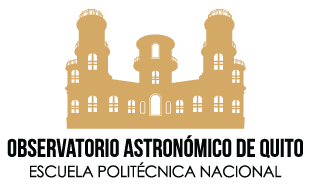
\includegraphics[scale=.25]{logo.png}
\end{center}
\end{minipage}\\
\rule[1mm]{170mm}{0.20mm}
\begin{center}
\textbf{\huge EFEM\'ERIDES ASTRON\'OMICAS 2020 \\}
%\vspace{0.5cm}
\end{center}
\section{ENERO}
\begin{center}
\begin{tabular}{ |l| l| l| }
\hline
 \textbf{Fecha} & \textbf{Hora (LT)} & \textbf{Evento}\\
 \hline
02/01/2020 & 10:16:15   &  Mercurio a 1.50$\degree$S de Júpiter. (Elongación mínima de los planetas: 4.6$\degree$)	  \\
02/01/2020 &  11:41:33   &  Mercurio a 1.50$\degree$ de Júpiter. (Elongación mínima de los planetas: 4.7$\degree$)	  \\
02/01/2020 &  23:45:26   &  Cuarto creciente (Distancia geocéntrica:403730 Km.)	  \\
04/01/2020 &  19:18:23   &  Urano a 4.43$\degree$ de la Luna. (Altura solar: -13.1$\degree$)	  \\
05/01/2020 &  02:47:54   &  Tierra en el perihelio. (Distancia heliocéntrica: 0.98324 U.A.)	  \\
10/01/2020 &  10:01:26   &  Mercurio en conjunción superior. (Distancia geocéntrica: 1.43034 U.A.)	  \\
10/01/2020 &  14:10:10   &  Eclipse penumbral de Luna Visibilidad:No visible Magnitud:-0.11	  \\
10/01/2020 &  14:21:18   &  Luna llena (Distancia geocéntrica:371543 Km.)	  \\
10/01/2020 &  20:13:54   &  Urano estacionario. (Elongación: 102.4$\degree$)	  \\
11/01/2020 &  23:31:33   &  Mercurio a 2.06$\degree$S de Saturno. (Elongación mínima de los planetas: 1.3$\degree$)	  \\
12/01/2020 &  04:51:06   &  Mercurio a 2.04$\degree$ de Saturno. (Elongación mínima de los planetas: 1.1$\degree$)	  \\
13/01/2020 &  10:18:32   &  Saturno en conjunción. (Distancia geocéntrica:11.01651 U.A.)	  \\
13/01/2020 &  15:21:03   &  Luna en el perigeo. (Distancia geocéntrica: 365958 Km | Iluminación: 87.9\%)	  \\
17/01/2020 &  07:58:26   &  Cuarto menguante (Distancia geocéntrica:371872 Km.)	  \\
22/01/2020 &  21:40:57   &  Ocultación de Júpiter por la Luna. DM: 0.382 Ilum: 3.3\%  \\
24/01/2020 &  16:42:00   &  Luna nueva (Distancia geocéntrica:395269 Km.)	  \\
25/01/2020 &  13:16:18   &  Mercurio a 1.63$\degree$N de la Luna. (Altura solar: 67.6$\degree$)	  \\
25/01/2020 &  16:22:17   &  Mercurio a 1.42$\degree$ de la Luna. (Altura solar: 29.3$\degree$)	  \\
27/01/2020 &  14:23:46   &  Venus a 0.08$\degree$S de Neptuno. (Elongación mínima de los planetas: 39.6$\degree$)	  \\
27/01/2020 &  15:00:23   &  Venus a 0.07$\degree$ de Neptuno. (Elongación mínima de los planetas: 39.6$\degree$)	  \\
29/01/2020 &  16:27:05   &  Luna en el apogeo. (Distancia geocéntrica: 405393 Km )\\
%\textcolor{blue!80!black}{31/01/2018} & \textcolor{blue!80!black}{08:29:52 }& 	\textcolor{blue!80!black}{Eclipse total de Luna Visibilidad:Sin final Magnitud: 1.32}	\\
\hline
\end{tabular}
\end{center}
%\vspace{0.5cm}
\textbf{NOTA:  }\textit{Todos los eventos son calculados para la ubicaci\'on de la ciudad de Quito, y las horas se encuentran en hora local(LT=UTC-5)}
%\vspace{0.7cm}
\newpage
\section{FEBRERO}
\begin{center}
\begin{tabular}{ |l| l| l| }
\hline
 \textbf{Fecha} & \textbf{Hora} & \textbf{Evento}\\
 \hline
01/02/2020 &  20:41:41   &  Cuarto creciente (Distancia geocéntrica:399314 Km.)	  \\
05/02/2020 &  09:00:44   &  Máxima extensión iluminada de Mercurio. (EI: $21.8"^2$ A.Fase: 63.78$\degree$ ) 	  \\
09/02/2020 &  02:33:18   &  Luna llena (Distancia geocéntrica:362477 Km.)	  \\
10/02/2020 &  08:45:45   &  Mercurio en máxima elongación este. (Elongación: 18.20$\degree$)	  \\
10/02/2020 &  15:27:54   &  Luna en el perigeo. (Distancia geocéntrica: 360461 Km | Iluminación: 96.4\%)	  \\
12/02/2020 &  00:05:12   &  Mercurio en el perihelio. (Distancia heliocéntrica: 0.30749 U.A.)	  \\
15/02/2020 &  17:17:13   &  Cuarto menguante (Distancia geocéntrica:376138 Km.)	  \\
16/02/2020 &  19:47:12   &  Mercurio estacionario. (Elongación: 15.3$\degree$)	  \\
18/02/2020 &  08:06:38   &  Marte a 0.39$\degree$S de la Luna. (Altura solar: 24.2$\degree$)	  \\
18/02/2020 &  08:21:14   &  Marte a 0.39$\degree$ de la Luna. (Altura solar: 27.8$\degree$)	  \\
18/02/2020 &  08:24:22   &  Ocultación de Marte por la Luna. DM: 0.799 Ilum: 23.5\%	  \\
19/02/2020 &  14:40:05   &  Ocultación de Júpiter por la Luna. DM: 0.998 Ilum: 13.6\%	  \\
20/02/2020 &  07:20:05   &  Saturno a 2.08$\degree$ de la Luna. (Altura solar: 12.9$\degree$)	  \\
20/02/2020 &  07:27:33   &  Saturno a 2.08$\degree$N de la Luna. (Altura solar: 14.8$\degree$)	  \\
23/02/2020 &  10:32:02   &  Luna nueva (Distancia geocéntrica:403387 Km.)	  \\
23/02/2020 &  14:33:26   &  Mercurio a 8.65$\degree$N de la Luna. (Altura solar: 57.2$\degree$)	  \\
24/02/2020 &  08:21:20   &  Neptuno a 4.43$\degree$N de la Luna. (Altura solar: 28.2$\degree$)	  \\
24/02/2020 &  16:18:05   &  Neptuno a 3.74$\degree$ de la Luna. (Altura solar: 31.9$\degree$)	  \\
25/02/2020 &  20:38:08   &  Mercurio en conjunción inferior. (Distancia geocéntrica: 0.63691 U.A.)	  \\
26/02/2020 &  06:34:15   &  Luna en el apogeo. (Distancia geocéntrica: 406278 Km | Iluminación: 7.3\%)	  \\
27/02/2020 &  16:55:38   &  Venus a 5.83$\degree$ de la Luna. (Altura solar: 22.6$\degree$)	  \\
\hline
\end{tabular}
\end{center}
\vspace{1cm}
\textbf{NOTA:  }\textit{Todos los eventos son calculados para la ubicaci\'on de la ciudad de Quito, y las horas se encuentran en hora local(LT=UTC-5)}
\vspace{0.7cm}
\newpage
\section{MARZO}
\begin{center}
\begin{tabular}{ |l| l| l| }
\hline
 \textbf{Fecha} & \textbf{Hora} & \textbf{Evento}\\
 \hline
02/03/2020 &  14:57:23   &  Cuarto creciente (Distancia geocéntrica:392070 Km.)	  \\
08/03/2020 &  07:24:33   &  Neptuno en conjunción. (Distancia geocéntrica:30.92438 U.A.)	  \\
08/03/2020 &  14:37:49   &  Venus a 2.21$\degree$ de Urano. (Elongación mínima de los planetas: 45.3$\degree$)	  \\
09/03/2020 &  09:28:04   &  Venus a 2.41$\degree$N de Urano. (Elongación mínima de los planetas: 44.6$\degree$)	  \\
09/03/2020 &  12:47:46   &  Luna llena (Distancia geocéntrica:357400 Km.)	  \\
09/03/2020 &  22:42:47   &  Mercurio estacionario. (Elongación: 21.9$\degree$)	  \\
10/03/2020 &  01:29:51   &  Luna en el perigeo. (Distancia geocéntrica: 357122 Km | Iluminación: 99.4\%)	  \\
16/03/2020 &  04:34:12   &  Cuarto menguante (Distancia geocéntrica:382671 Km.)	  \\
18/03/2020 &  03:11:12   &  Júpiter a 1.71$\degree$ de la Luna. (Altura solar: -47.4$\degree$)	  \\
18/03/2020 &  03:24:35   &  Ocultación de Marte por la Luna. DM: 0.795 Ilum: 30.5\%	  \\
18/03/2020 &  03:38:29   &  Júpiter a 1.72$\degree$N de la Luna. (Altura solar: -40.6$\degree$)	  \\
19/03/2020 &  21:09:04   &  Venus en el perihelio. (Distancia heliocéntrica: 0.71845 U.A.)	  \\
19/03/2020 &  22:49:36   &  Equinoccio de marzo.	  \\
20/03/2020 &  01:19:14   &  Marte a 0.71$\degree$S de Júpiter. (Elongación mínima de los planetas: 67.3$\degree$)	  \\
20/03/2020 &  06:34:48   &  Marte a 0.71$\degree$ de Júpiter. (Elongación mínima de los planetas: 67.5$\degree$)	  \\
21/03/2020 &  14:34:22   &  Mercurio a 3.45$\degree$N de la Luna. (Altura solar: 56.6$\degree$)	  \\
21/03/2020 &  17:57:08   &  Máxima extensión iluminada de Mercurio. (EI: $22.8"^2$ A.Fase: 90.95$\degree$ ) 	  \\
23/03/2020 &  20:55:59   &  Mercurio en máxima elongación oeste. (Elongación: 27.78$\degree$)	  \\
24/03/2020 &  04:28:15   &  Luna nueva (Distancia geocéntrica:406672 Km.)	  \\
24/03/2020 &  10:22:57   &  Luna en el apogeo. (Distancia geocéntrica: 406692 Km | Iluminación: 0.2\%)	  \\
24/03/2020 &  16:57:41   &  Venus en máxima elongación este. (Elongación: 46.08$\degree$)	  \\
26/03/2020 &  17:05:59   &  Urano a 3.73$\degree$N de la Luna. (Altura solar: 18.4$\degree$)	  \\
26/03/2020 &  20:01:59   &  Urano a 3.46$\degree$ de la Luna. (Altura solar: -25.2$\degree$)	  \\
26/03/2020 &  23:42:32   &  Mercurio en el afelio. (Distancia heliocéntrica: 0.46670 U.A.)	  \\
28/03/2020 &  14:10:54   &  Venus a 6.67$\degree$ de la Luna. (Altura solar: 61.8$\degree$)	  \\ 
31/03/2020 &  05:56:43   &  Marte a 0.92$\degree$S de Saturno. (Elongación mínima de los planetas: 70.6$\degree$)	  \\
31/03/2020 &  13:31:20   &  Marte a 0.91$\degree$ de Saturno. (Elongación mínima de los planetas: 70.8$\degree$)	\\
\hline
\end{tabular}
\end{center}
\vspace{1cm}
\textbf{NOTA:  }\textit{Todos los eventos son calculados para la ubicaci\'on de la ciudad de Quito, y las horas se encuentran en hora local(LT=UTC-5)}
\vspace{0.7cm}
\newpage
\section{ABRIL}
\begin{center}
\begin{tabular}{ |l| l| l| }
\hline
 \textbf{Fecha} & \textbf{Hora} & \textbf{Evento}\\
 \hline
01/04/2020 &  05:21:16   &  Cuarto creciente (Distancia geocéntrica:384056 Km.)	  \\
03/04/2020 &  10:18:55   &  Mercurio a 1.42$\degree$S de Neptuno. (Elongación mínima de los planetas: 25.0$\degree$)	  \\
03/04/2020 &  20:14:39   &  Mercurio a 1.33$\degree$ de Neptuno. (Elongación mínima de los planetas: 25.4$\degree$)	  \\
07/04/2020 &  13:08:38   &  Luna en el perigeo. (Distancia geocéntrica: 356907 Km | Iluminación: 99.6\%)	  \\
07/04/2020 &  21:35:06   &  Luna llena (Distancia geocéntrica:357030 Km.)	  \\
14/04/2020 &  17:56:08   &  Cuarto menguante (Distancia geocéntrica:390383 Km.)	  \\
15/04/2020 &  02:31:45   &  Saturno a 2.74$\degree$ de la Luna. (Altura solar: -54.2$\degree$)	  \\
15/04/2020 &  02:41:32   &  Saturno a 2.74$\degree$N de la Luna. (Altura solar: -51.8$\degree$)	  \\
20/04/2020 &  14:00:11   &  Luna en el apogeo. (Distancia geocéntrica: 406462 Km | Iluminación: 5.0\%)	  \\
21/04/2020 &  13:30:10   &  Mercurio a 2.87$\degree$N de la Luna. (Altura solar: 67.1$\degree$)	  \\
21/04/2020 &  17:09:07   &  Mercurio a 2.49$\degree$ de la Luna. (Altura solar: 15.5$\degree$)	  \\
22/04/2020 &  21:25:52   &  Luna nueva (Distancia geocéntrica:404547 Km.)	  \\
26/04/2020 &  04:02:52   &  Urano en conjunción. (Distancia geocéntrica:20.81054 U.A.)	  \\
26/04/2020 &  14:37:52   &  Venus a 5.73$\degree$ de la Luna. (Altura solar: 51.2$\degree$)	  \\ 
27/04/2020 &  20:07:38   &  Máxima extensión iluminada de Venus. (EI: $297.7"^2$ A.Fase: 116.70$\degree$) 	  \\
30/04/2020 &  15:38:22   &  Cuarto creciente (Distancia geocéntrica:377093 Km.) \\
30/04/2020 &  21:26:47   &  Mercurio a 0.32$\degree$S de Urano. (Elongación mínima de los planetas: 4.3$\degree$)	  \\
30/04/2020 &  22:40:42   &  Mercurio a 0.30$\degree$ de Urano. (Elongación mínima de los planetas: 4.4$\degree$)\\	
\hline
\end{tabular}
\end{center}
\vspace{1cm}
\textbf{NOTA:  }\textit{Todos los eventos son calculados para la ubicaci\'on de la ciudad de Quito, y las horas se encuentran en hora local(LT=UTC-5)}
\vspace{0.7cm}
\newpage
\section{MAYO}
\begin{center}
\begin{tabular}{ |l| l| l| }
\hline
 \textbf{Fecha} & \textbf{Hora} & \textbf{Evento}\\
 \hline
04/05/2020 &  16:28:20   &  Mercurio en conjunción superior. (Distancia geocéntrica: 1.32469 U.A.)	  \\
05/05/2020 &  22:02:43   &  Luna en el perigeo. (Distancia geocéntrica: 359654 Km | Iluminación: 97.3\%)	  \\
07/05/2020 &  05:45:14   &  Luna llena (Distancia geocéntrica:361183 Km.)	  \\
09/05/2020 &  23:20:18   &  Mercurio en el perihelio. (Distancia heliocéntrica: 0.30749 U.A.)	  \\
10/05/2020 &  20:44:43   &  Saturno estacionario. (Elongación: 108.9$\degree$)	  \\
12/05/2020 &  04:34:01   &  Júpiter a 2.63$\degree$N de la Luna. (Altura solar: -22.5$\degree$)	  \\
12/05/2020 &  07:21:37   &  Júpiter a 2.53$\degree$ de la Luna. (Altura solar: 16.9$\degree$)	  \\
13/05/2020 &  01:40:19   &  Venus estacionario. (Elongación: 29.2$\degree$)	  \\
14/05/2020 &  03:23:49   &  Máxima extensión iluminada de Mercurio. (EI: $20.7"^2$ A.Fase: 38.77$\degree$ ) 	  \\
14/05/2020 &  08:37:43   &  Júpiter estacionario. (Elongación: 117.0$\degree$)	  \\
14/05/2020 &  09:02:44   &  Cuarto menguante (Distancia geocéntrica:397606 Km.)	  \\
16/05/2020 &  11:39:49   &  Neptuno a 4.19$\degree$N de la Luna. (Altura solar: 69.1$\degree$)	  \\
18/05/2020 &  02:44:31   &  Luna en el apogeo. (Distancia geocéntrica: 405583 Km | Iluminación: 17.3\%)	  \\
20/05/2020 &  10:27:47   &  Urano a 3.76$\degree$N de la Luna. (Altura solar: 57.6$\degree$)	  \\
20/05/2020 &  15:01:09   &  Urano a 3.24$\degree$ de la Luna. (Altura solar: 43.6$\degree$)	  \\
22/05/2020 &  02:55:30   &  Mercurio a 0.89$\degree$S de Venus. (Elongación mínima de los planetas: 18.6$\degree$)	  \\
22/05/2020 &  03:41:11   &  Mercurio a 0.88$\degree$ de Venus. (Elongación mínima de los planetas: 18.6$\degree$)	  \\
22/05/2020 &  12:38:52   &  Luna nueva (Distancia geocéntrica:397761 Km.)	  \\   
29/05/2020 &  22:29:56   &  Cuarto creciente (Distancia geocéntrica:372236 Km.)	  \\ 
\hline
\end{tabular}
\end{center}
\vspace{1cm}
\textbf{NOTA:  }\textit{Todos los eventos son calculados para la ubicaci\'on de la ciudad de Quito, y las horas se encuentran en hora local(LT=UTC-5)}
\vspace{0.7cm}
\newpage
\section{JUNIO}
\begin{center}
\begin{tabular}{ |l| l| l| }
\hline
 \textbf{Fecha} & \textbf{Hora (LT)} & \textbf{Evento}\\
 \hline
02/06/2020 &  22:38:31   &  Luna en el perigeo. (Distancia geocéntrica: 364366 Km | Iluminación: 90.4\%)	  \\
03/06/2020 &  12:37:35   &  Venus en conjunción inferior. (Distancia geocéntrica: 0.28858 U.A.)	  \\
04/06/2020 &  07:57:41   &  Mercurio en máxima elongación este. (Elongación: 23.60$\degree$)	  \\
05/06/2020 &  14:12:23   &  Luna llena (Distancia geocéntrica:369005 Km.)	  \\
05/06/2020 &  14:24:59   &  Eclipse penumbral de Luna Visibilidad:No visible Magnitud:-0.40	  \\
12/06/2020 &  07:24:43   &  Marte a 1.74$\degree$S de Neptuno. (Elongación mínima de los planetas: 91.1$\degree$)	  \\
13/06/2020 &  01:23:43   &  Cuarto menguante (Distancia geocéntrica:402617 Km.)	  \\
13/06/2020 &  09:13:22   &  Marte a 1.63$\degree$ de Neptuno. (Elongación mínima de los planetas: 92.1$\degree$)	  \\
14/06/2020 &  19:56:36   &  Luna en el apogeo. (Distancia geocéntrica: 404595 Km | Iluminación: 33.6\%)	  \\
17/06/2020 &  23:52:52   &  Mercurio estacionario. (Elongación: 17.4$\degree$)	  \\
19/06/2020 &  03:32:00   &  Ocultación de Venus por la Luna. DM: 0.776 Ilum: 3.9\%	  \\
20/06/2020 &  16:43:40   &  Solsticio de junio.  \\
21/06/2020 &  01:40:06   &  Eclipse de sol DM: 0.121 TG: Anular TO: No visible   \\
21/06/2020 &  01:41:28   &  Luna nueva (Distancia geocéntrica:387967 Km.)	  \\ 
22/06/2020 &  16:09:39   &  Neptuno estacionario. (Elongación: 100.9$\degree$)	  \\
22/06/2020 &  22:58:03   &  Mercurio en el afelio. (Distancia heliocéntrica: 0.46670 U.A.)	  \\
25/06/2020 &  01:47:03   &  Venus estacionario. (Elongación: 29.0$\degree$)	  \\
28/06/2020 &  03:15:43   &  Cuarto creciente (Distancia geocéntrica:369879 Km.)	  \\
29/06/2020 &  21:12:45   &  Luna en el perigeo. (Distancia geocéntrica: 368958 Km | Iluminación: 69.8\%)	  \\ 
30/06/2020 &  21:45:39   &  Mercurio en conjunción inferior. (Distancia geocéntrica: 0.56253 U.A.)	  \\
\hline
\end{tabular}
\end{center}
\vspace{1cm}
\textbf{NOTA:  }\textit{Todos los eventos son calculados para la ubicaci\'on de la ciudad de Quito, y las horas se encuentran en hora local(LT=UTC-5)}
\vspace{0.7cm}
\newpage
\section{JULIO}
\begin{center}
\begin{tabular}{ |l| l| l| }
\hline
 \textbf{Fecha} & \textbf{Hora (LT)} & \textbf{Evento}\\
 \hline
04/07/2020 &  06:34:44   &  Tierra en el afelio. (Distancia heliocéntrica: 1.01669 U.A.)	  \\
04/07/2020 &  23:30:13   &  Eclipse penumbral de Luna Visibilidad:Todo el eclipse Magnitud:-0.64	  \\
04/07/2020 &  23:44:24   &  Luna llena (Distancia geocéntrica:379149 Km.)	  \\
06/07/2020 &  05:04:09   &  Saturno a 2.59$\degree$N de la Luna. (Altura solar: -16.8$\degree$)	  \\
06/07/2020 &  06:45:13   &  Saturno a 2.44$\degree$ de la Luna. (Altura solar: 6.1$\degree$)	  \\
10/07/2020 &  00:53:58   &  Neptuno a 4.83$\degree$N de la Luna. (Altura solar: -66.3$\degree$)	  \\
10/07/2020 &  02:38:19   &  Máxima extensión iluminada de Venus. (EI: $292.3"^2$ A.Fase: 117.34$\degree$) 	  \\
10/07/2020 &  08:40:42   &  Neptuno a 3.91$\degree$ de la Luna. (Altura solar: 32.3$\degree$)	  \\
10/07/2020 &  09:43:52   &  Venus en el afelio. (Distancia heliocéntrica: 0.72823 U.A.)	  \\
12/07/2020 &  03:21:11   &  Mercurio estacionario. (Elongación: 15.6$\degree$)	  \\
12/07/2020 &  14:26:32   &  Luna en el apogeo. (Distancia geocéntrica: 404199 Km | Iluminación: 51.7\%)	  \\
12/07/2020 &  18:29:02   &  Cuarto menguante (Distancia geocéntrica:404181 Km.)	  \\
14/07/2020 &  02:46:53   &  Júpiter en oposición. (Distancia geocéntrica: 4.13950 U.A.)	  \\
14/07/2020 &  06:28:35   &  Urano a 3.65$\degree$N de la Luna. (Altura solar: 2.2$\degree$)	  \\
14/07/2020 &  11:10:20   &  Urano a 3.11$\degree$ de la Luna. (Altura solar: 62.4$\degree$)	  \\
20/07/2020 &  12:32:58   &  Luna nueva (Distancia geocéntrica:377190 Km.)	  \\
20/07/2020 &  17:14:30   &  Saturno en oposición. (Distancia geocéntrica: 8.99470 U.A.)	  \\ 
22/07/2020 &  10:02:38   &  Mercurio en máxima elongación oeste. (Elongación: 20.13$\degree$)	  \\ 
25/07/2020 &  00:01:46   &  Luna en el perigeo. (Distancia geocéntrica: 368361 Km | Iluminación: 24.6\%)	  \\
27/07/2020 &  07:32:35   &  Cuarto creciente (Distancia geocéntrica:370139 Km.)	  \\ 
\hline
\end{tabular}
\end{center}
\vspace{1cm}
\textbf{NOTA:  }\textit{Todos los eventos son calculados para la ubicaci\'on de la ciudad de Quito, y las horas se encuentran en hora local(LT=UTC-5)}
\vspace{0.7cm}
\newpage
\section{AGOSTO}
\begin{center}
\begin{tabular}{ |l| l| l| }
\hline
 \textbf{Fecha} & \textbf{Hora (LT)} & \textbf{Evento}\\
 \hline
03/08/2020 &  04:02:57   &  Marte en el perihelio. (Distancia heliocéntrica: 1.38138 U.A.)	  \\
03/08/2020 &  10:58:47   &  Luna llena (Distancia geocéntrica:389877 Km.)	  \\
04/08/2020 &  15:07:40   &  Máxima extensión iluminada de Mercurio. (EI: $20.8"^2 $A.Fase: 50.13$\degree$) 	  \\
05/08/2020 &  22:37:07   &  Mercurio en el perihelio. (Distancia heliocéntrica: 0.30750 U.A.)	  \\
09/08/2020 &  01:36:10   &  Marte a 0.98$\degree$N de la Luna. (Altura solar: -65.4$\degree$)	  \\
09/08/2020 &  03:38:35   &  Ocultación de Marte por la Luna. DM: 0.765 Ilum: 71.6\% 	  \\
09/08/2020 &  03:48:25   &  Marte a 0.73$\degree$ de la Luna. (Altura solar: -35.9$\degree$)	  \\
09/08/2020 &  08:50:04   &  Luna en el apogeo. (Distancia geocéntrica: 404659 Km | Iluminación: 69.7\%)	  \\
11/08/2020 &  11:44:48   &  Cuarto menguante (Distancia geocéntrica:401869 Km.)	  \\
12/08/2020 &  18:59:06   &  Venus en máxima elongación oeste. (Elongación: 45.79$\degree$)	  \\
15/08/2020 &  04:05:32   &  Venus a 4.16$\degree$ de la Luna. (Altura solar: -31.8$\degree$)	  \\
15/08/2020 &  04:52:07   &  Urano estacionario. (Elongación: 102.3$\degree$)	  \\
15/08/2020 &  07:01:23   &  Venus a 4.31$\degree$S de la Luna. (Altura solar: 10.5$\degree$)	  \\
17/08/2020 &  09:53:32   &  Mercurio en conjunción superior. (Distancia geocéntrica: 1.35397 U.A.)	  \\
18/08/2020 &  21:41:40   &  Luna nueva (Distancia geocéntrica:367384 Km.)	  \\ 
21/08/2020 &  05:57:03   &  Luna en el perigeo. (Distancia geocéntrica: 363513 Km | Iluminación: 7.9\%)	  \\
25/08/2020 &  12:57:38   &  Cuarto creciente (Distancia geocéntrica:373062 Km.)	  \\
28/08/2020 &  20:15:10   &  Júpiter a 1.80$\degree$N de la Luna. (Altura solar: -29.3$\degree$)	  \\
28/08/2020 &  20:32:58   &  Júpiter a 1.80$\degree$ de la Luna. (Altura solar: -33.7$\degree$)	  \\ 
\hline
\end{tabular}
\end{center}
\vspace{1cm}
\textbf{NOTA:  }\textit{Todos los eventos son calculados para la ubicaci\'on de la ciudad de Quito, y las horas se encuentran en hora local(LT=UTC-5)}
\vspace{0.7cm}
\newpage
\section{SEPTIEMBRE}
\begin{center}
\begin{tabular}{ |l| l| l| }
\hline
 \textbf{Fecha} & \textbf{Hora (LT)} & \textbf{Evento}\\
 \hline
02/09/2020 &  00:22:06   &  Luna llena (Distancia geocéntrica:399203 Km.)	  \\
05/09/2020 &  21:49:10   &  Marte a 0.33$\degree$N de la Luna. (Altura solar: -53.6$\degree$)	  \\
05/09/2020 &  22:11:03   &  Marte a 0.29$\degree$ de la Luna. (Altura solar: -59.0$\degree$)	  \\
05/09/2020 &  23:44:50   &  Ocultación de Marte por la Luna. DM: 0.027 Ilum: 85.9\%   \\
06/09/2020 &  01:28:56   &  Luna en el apogeo. (Distancia geocéntrica: 405607 Km | Iluminación: 85.5\%)	  \\
07/09/2020 &  02:51:15   &  Urano a 3.14$\degree$ de la Luna. (Altura solar: -49.6$\degree$)	  \\
09/09/2020 &  17:14:16   &  Marte estacionario. (Elongación: 139.4$\degree$)	  \\
10/09/2020 &  04:25:44   &  Cuarto menguante (Distancia geocéntrica:396234 Km.)	  \\
11/09/2020 &  15:10:54   &  Neptuno en oposición. (Distancia geocéntrica:28.92250 U.A.)	  \\
12/09/2020 &  19:26:08   &  Júpiter estacionario. (Elongación: 116.7$\degree$)	  \\
17/09/2020 &  06:00:14   &  Luna nueva (Distancia geocéntrica:360210 Km.)	  \\
18/09/2020 &  08:48:01   &  Luna en el perigeo. (Distancia geocéntrica: 359082 Km | Iluminación: 2.1\%)	  \\
18/09/2020 &  18:47:07   &  Mercurio a 5.98$\degree$S de la Luna. (Altura solar: -9.3$\degree$)	  \\ 
18/09/2020 &  22:15:02   &  Mercurio en el afelio. (Distancia heliocéntrica: 0.46670 U.A.)	  \\ 
22/09/2020 &  08:30:40   &  Equinoccio de septiembre.	  \\
23/09/2020 &  20:54:52   &  Cuarto creciente (Distancia geocéntrica:378509 Km.)	  \\
25/09/2020 &  13:52:43   &  Saturno a 2.45$\degree$N de la Luna. (Altura solar: 63.2$\degree$)	  \\
28/09/2020 &  22:57:58   &  Saturno estacionario. (Elongación: 108.9$\degree$)	  \\
29/09/2020 &  19:04:03   &  Neptuno a 4.61$\degree$N de la Luna. (Altura solar: -14.5$\degree$)	  \\
30/09/2020 &  02:50:22   &  Neptuno a 3.72$\degree$ de la Luna. (Altura solar: -48.0$\degree$)	  \\ 
\hline
\end{tabular}
\end{center}
\vspace{1cm}
\textbf{NOTA:  }\textit{Todos los eventos son calculados para la ubicaci\'on de la ciudad de Quito, y las horas se encuentran en hora local(LT=UTC-5)}
\vspace{0.7cm}
\newpage
\section{OCTUBRE}
\begin{center}
\begin{tabular}{ |l| l| l| }
\hline
 \textbf{Fecha} & \textbf{Hora (LT)} & \textbf{Evento}\\
 \hline
01/10/2020 &  10:54:11   &  Mercurio en máxima elongación este. (Elongación: 25.82$\degree$)	  \\
01/10/2020 &  16:05:17   &  Luna llena (Distancia geocéntrica:405149 Km.)	  \\
02/10/2020 &  20:40:32   &  Marte a 1.04$\degree$N de la Luna. (Altura solar: -38.9$\degree$)	  \\
02/10/2020 &  22:16:00   &  Marte a 0.86$\degree$ de la Luna. (Altura solar: -62.8$\degree$)	  \\
02/10/2020 &  23:00:10   &  Ocultación de Marte por la Luna. DM: 0.738 Ilum: 98.4\% 	  \\
03/10/2020 &  12:22:24   &  Luna en el apogeo. (Distancia geocéntrica: 406321 Km | Iluminación: 96.9\%)	  \\
04/10/2020 &  00:14:41   &  Máxima extensión iluminada de Mercurio. (EI: $21.9"^2 $A.Fase: 83.94$\degree$) 	  \\
04/10/2020 &  05:35:14   &  Urano a 2.77$\degree$N de la Luna. (Altura solar: -6.3$\degree$)	  \\
04/10/2020 &  07:35:58   &  Urano a 2.60$\degree$ de la Luna. (Altura solar: 23.3$\degree$)	  \\
09/10/2020 &  19:39:32   &  Cuarto menguante (Distancia geocéntrica:388736 Km.)	  \\
13/10/2020 &  18:18:39   &  Marte en oposición. (Distancia geocéntrica: 0.41923 U.A.)	  \\
13/10/2020 &  19:58:25   &  Mercurio estacionario. (Elongación: 20.8$\degree$)	  \\
16/10/2020 &  14:31:03   &  Luna nueva (Distancia geocéntrica:356943 Km.)	  \\
16/10/2020 &  18:46:17   &  Luna en el perigeo. (Distancia geocéntrica: 356912 Km | Iluminación: 0.2\%)	  \\
17/10/2020 &  14:06:01   &  Mercurio a 6.47$\degree$S de la Luna. (Altura solar: 57.1$\degree$)	  \\
17/10/2020 &  18:26:46   &  Mercurio a 5.86$\degree$ de la Luna. (Altura solar: -6.3$\degree$)	  \\ 
23/10/2020 &  08:22:56   &  Cuarto creciente (Distancia geocéntrica:385858 Km.)	  \\
25/10/2020 &  13:16:20   &  Mercurio en conjunción inferior. (Distancia geocéntrica: 0.67070 U.A.)	  \\
30/10/2020 &  13:45:26   &  Luna en el apogeo. (Distancia geocéntrica: 406394 Km | Iluminación: 99.3\%)	  \\
30/10/2020 &  18:03:39   &  Venus en el perihelio. (Distancia heliocéntrica: 0.71841 U.A.)	  \\
31/10/2020 &  09:49:10   &  Luna llena (Distancia geocéntrica:406167 Km.)	  \\
31/10/2020 &  10:38:58   &  Urano en oposición. (Distancia geocéntrica:18.78761 U.A.)	  \\
\hline
\end{tabular}
\end{center}
\vspace{1cm}
\textbf{NOTA:  }\textit{Todos los eventos son calculados para la ubicaci\'on de la ciudad de Quito, y las horas se encuentran en hora local(LT=UTC-5)}
\vspace{0.7cm}
\newpage
\section{NOVIEMBRE}
\begin{center}
\begin{tabular}{ |l| l| l| }
\hline
 \textbf{Fecha} & \textbf{Hora (LT)} & \textbf{Evento}\\
 \hline
01/11/2020 &  21:53:15   &  Mercurio en el perihelio. (Distancia heliocéntrica: 0.30750 U.A.)	  \\
03/11/2020 &  12:43:27   &  Mercurio estacionario. (Elongación: 16.0$\degree$)	  \\
08/11/2020 &  08:46:07   &  Cuarto menguante (Distancia geocéntrica:381211 Km.)	  \\
10/11/2020 &  11:52:26   &  Mercurio en máxima elongación oeste. (Elongación: 19.10$\degree$)	  \\
13/11/2020 &  04:33:46   &  Máxima extensión iluminada de Mercurio. (EI: $21.5"^2 $A.Fase: 68.53$\degree$) 	  \\
13/11/2020 &  19:34:19   &  Marte estacionario. (Elongación: 143.1$\degree$)	  \\
14/11/2020 &  06:43:08   &  Luna en el perigeo. (Distancia geocéntrica: 357837 Km | Iluminación: 0.9\%)	  \\
15/11/2020 &  00:07:11   &  Luna nueva (Distancia geocéntrica:358346 Km.)	  \\  
21/11/2020 &  23:45:02   &  Cuarto creciente (Distancia geocéntrica:393809 Km.)	  \\
25/11/2020 &  22:18:26   &  Marte a 4.51$\degree$ de la Luna. (Altura solar: -56.9$\degree$)	  \\
26/11/2020 &  19:28:36   &  Luna en el apogeo. (Distancia geocéntrica: 405894 Km | Iluminación: 90.0\%)	  \\
28/11/2020 &  17:27:08   &  Neptuno estacionario. (Elongación: 101.0$\degree$)	  \\
30/11/2020 &  04:29:40   &  Luna llena (Distancia geocéntrica:401726 Km.)	  \\
30/11/2020 &  04:42:45   &  Eclipse penumbral de Luna Visibilidad:Sin final Magnitud:-0.26	\\
\hline
\end{tabular}
\end{center}
\vspace{1cm}
\textbf{NOTA:  }\textit{Todos los eventos son calculados para la ubicaci\'on de la ciudad de Quito, y las horas se encuentran en hora local(LT=UTC-5)}
\vspace{0.7cm}
\newpage
\section{DICIEMBRE}
\begin{center}
\begin{tabular}{ |l| l| l| }
\hline
 \textbf{Fecha} & \textbf{Hora (LT)} & \textbf{Evento}\\
 \hline
07/12/2020 &  19:36:35   &  Cuarto menguante (Distancia geocéntrica:375148 Km.)	  \\
12/12/2020 &  15:42:02   &  Luna en el perigeo. (Distancia geocéntrica: 361773 Km | Iluminación: 4.7\%)	  \\
12/12/2020 &  16:06:15   &  Ocultación de Venus por la Luna. DM: 0.745 Ilum: 4.6\% 	  \\
14/12/2020 &  05:51:37   &  Ocultación de Mercurio por la Luna. DM: 0.952 Ilum: 0.1\% 	  \\
14/12/2020 &  11:13:28   &  Eclipse de sol DM: 0.294 TG: Total TO: No visible 	  \\
14/12/2020 &  11:16:32   &  Luna nueva (Distancia geocéntrica:364413 Km.)	  \\ 
15/12/2020 &  21:30:48   &  Mercurio en el afelio. (Distancia heliocéntrica: 0.46670 U.A.)	  \\
19/12/2020 &  22:06:41   &  Mercurio en conjunción superior. (Distancia geocéntrica: 1.44727 U.A.)	  \\
20/12/2020 &  13:21:05   &  Neptuno a 4.98$\degree$N de la Luna. (Altura solar: 61.4$\degree$)	  \\
20/12/2020 &  21:32:00   &  Neptuno a 4.04$\degree$ de la Luna. (Altura solar: -44.2$\degree$)	  \\
21/12/2020 &  05:02:17   &  Solsticio de diciembre.  \\
21/12/2020 &  08:29:34   &  Júpiter a 0.10$\degree$S de Saturno. (Elongación mínima de los planetas: 30.3$\degree$)	  \\
21/12/2020 &  13:20:35   &  Júpiter a 0.10$\degree$ de Saturno. (Elongación mínima de los planetas: 30.1$\degree$)	  \\
21/12/2020 &  18:41:12   &  Cuarto creciente (Distancia geocéntrica:400513 Km.)	  \\
23/12/2020 &  21:44:29   &  Marte a 4.95$\degree$ de la Luna. (Altura solar: -46.5$\degree$)	  \\
24/12/2020 &  11:31:21   &  Luna en el apogeo. (Distancia geocéntrica: 405012 Km | Iluminación: 74.6\%)	  \\
24/12/2020 &  15:50:00   &  Urano a 3.71$\degree$N de la Luna. (Altura solar: 32.8$\degree$)	  \\
24/12/2020 &  22:13:49   &  Urano a 2.91$\degree$ de la Luna. (Altura solar: -52.2$\degree$)	  \\
29/12/2020 &  22:28:10   &  Luna llena (Distancia geocéntrica:392772 Km.)	 \\
\hline
\end{tabular}
\end{center}

\vspace{1cm}
\textbf{NOTA:  }\textit{Todos los eventos son calculados para la ubicaci\'on de la ciudad de Quito, y las horas se encuentran en hora local(LT=UTC-5)}
\vspace{0.7cm}

\newpage
\section{LLuvias de Meteoros 2020}
\begin{table}[h!b!t!]
\begin{center}
\resizebox{18cm}{!} {
\begin{tabular}{|c|c|c|}
\hline 
\textbf{Nombre de la lluvia}&	\textbf{ Intervalo de Observaci\'on ( M\'aximo)}  &	\textbf{THZ}\\ 
\hline 
\textcolor{blue!80!black}{Cuadr\'antidas (QUA)} &	\textcolor{blue!80!black}{28 de Diciembre al 12 de Enero (4 de Enero, 03:32)} &	\textcolor{blue!80!black}{110}\\ 
\hline 
%$\alpha$-Cent\'auridas (ACE) &	29 de Enero al 22 de Febrero (8 de Febrero, 07:56 ) & 6\\ 
%\hline 
%$\gamma$-N\'ormidas (GNO) &	26 de Febrero al 23 de Marzo (13 de Marzo, 22:34) & 8\\ 
%\hline 
\textcolor{blue!80!black}{L\'iridas (LYR)} &	\textcolor{blue!80!black}{14 de Abril al 30 de Abril (22 de Abril, 01:40)} & 	\textcolor{blue!80!black}{18}\\ 
\hline 
%$\pi$-P\'uppidas (PPU) &15 de Abril al 28 de Abril (24 de Abril de 2019, 01:34) &	var\\ 
%\hline 
\textcolor{blue!80!black}{$\eta$-Acu\'aridas (ETA)} & \textcolor{blue!80!black}{19 Abril – 28 Mayo (06 Mayo 03:11)} & 	\textcolor{blue!80!black}{50}\\ 
%\hline 
%Bootidas de Junio (JBO) & 22 Junio - 02 Julio (26 Junio 22:00 ) &	var\\ 
%\hline 
%Piscis Austr\'inidas (PAU) &	15 Julio - 10 Agosto (27 Julio 17:00) &	5\\ 
\hline 
\textcolor{blue!80!black}{$\delta$-Acu\'aridas Sur (SDA)} &	\textcolor{blue!80!black}{12 de Julio  al 23 de Agosto (30 de Julio, 18:30) }&\textcolor{blue!80!black}{25}\\ 
%\hline 
%$\alpha$-Capric\'ornidas (CAP) &	3 de Julio al 15 de Agosto(30 de Julio, 13:19) &	4\\ 
\hline 
\textcolor{blue!80!black}{Perseidas (PER}) 	& \textcolor{blue!80!black}{17 de Julio al 24 de Agosto (12 de Agosto de 2019, 08:13) }&	\textcolor{blue!80!black}{110}\\ 
%\hline 
%$\kappa$-C\'ignidas (KCG) &	4 de Agosto al 26 de Agosto (18 de Agosto, 07:57) &	3\\ 
%\hline 
%$\alpha$-Aur\'igidas (AUR) & 25 de Agosto al 8 de Septiembre( 1 de Septiembre, 10:21	) &	10\\ 
%\hline 
%Drac\'onidas (GIA) &	6 de Octubre al 10 de Octubre (8 de Octubre, 16:32) &	var\\ 
%\hline 
%$\epsilon$-Gem\'inidas (EGE) & 15 de Octubre al 28 de Octubre(18 de Octubre, 20:02) & 	 2\\ 
\hline
Ori\'onidas (ORI) & 	2 de Octubre al 7 de Noviembre (20 de Octubre, 00:35) &	20\\ 
\hline 
Le\'onidas (LEO) & 06 de Noviembre al 30 de Noviembre	 (17 de Noviembre, 05:54 ) &	15\\ 
%\hline  
%P'uppidas-V\'elidas (PUP) &	1 de Diciembre al 15 de Diciembre (7 de Diciembre, 11:34) &	10\\ 
\hline 
\textcolor{blue!80!black}{Gem\'inidas (GEM)} & \textcolor{blue!80!black}{	4 de Diciembre al 17 de Diciembre	 (14 de Diciembre, 19:48 )} &	\textcolor{blue!80!black}{20}\\ 
\hline 
\'Ursidas (URS) &	17 de Diciembre al 26 de Diciembre	 (22 de Diciembre, 04:13) & 10\\ 
\hline 
 \end{tabular} }
\end{center}
\end{table}

\vspace{0.5cm}
%\textbf{NOTA:  }\textit{Informaci\'on obtenida de \url{http://www.oan.es/servidorEfem/}}
\section{Eclipses Visibles desde Ecuador en el 2020}
\begin{itemize}
\item 04/07/2020 (23:30:13).- Eclipse penumbral de Luna (Visible todo el eclipse).
\item 30/11/2020 (04:42:45).- Eclipse penumbral de Luna (Visible sin final).
\end{itemize}
\section{Equinoccios y Solsticios 2020}
\begin{itemize}
\item 19/03/2020 (22:49:36).- Equinoccio de marzo.
\item 20/06/2020 (16:43:40).- Solsticio de junio.
\item 22/09/2020 (08:30:40).- Equinoccio de septiembre.
\item 21/12/2020 (05:02:17).- Solsticio de diciembre.
\end{itemize}
\newpage
\section{Diccionario Astron\'omico}

\subsection{Fases Lunares}
\begin{itemize}
\item [i.-]\textbf{Luna Nueva .-} La Luna se enceuntra entre la Tierra y el Sol y por lo tanto no la vemos.

\item[ii.-]\textbf{Cuarto Creciente.-} La Luna, la Tierra y el Sol forman un \'angulo recto, por lo que se puede observar en el cielo la mitad de la Luna, en su per\'iodo de crecimiento.

\item[iii.-]\textbf{Luna Llena.-} Ocurre cuando La Tierra se ubica entre el Sol y la Luna; \'esta recibe los rayos del sol en su cara visible, por lo tanto, se ve completa.
\item [iv.-]\textbf{ Cuarto Menguante.-} los tres cuerpos vuelven a formar \'angulo recto, por lo que se puede observar en el cielo la otra mitad de la cara lunar.

\end{itemize}
\subsection{Posici\'on}
\begin{itemize}
\item \textbf{Apogeo.-} Es el punto de la \'orbita en el cual el objeto se encuentra m\'as alejado al centro de la Tierra.
\item \textbf{Perigeo.-} Es el punto de la \'orbita en el cual el objeto se encuentra m\'as cercano al centro de la Tierra.
\item \textbf{Afelio.-} Es el punto de m\'axima distancia de un cuerpo al Sol.
\item \textbf{Perihelio.-} Es el punto de m'inima distancia de un cuerpo al Sol.
\item \textbf{Elongaci\'on.-} Es la distancia angular de un planeta al Sol, visto desde la Tierra.
\item \textbf{Conjunci\'on.-} Dos astros est\'an en conjunci\'on cuando se hallan en la misma longitud celeste. Los planetas cuya \'orbita es interior con respecto a la de la Tierra (Mercurio y Venus), pueden estar en conjunci\'on inferior cuando se encuentran entre el Sol y la Tierra, o en conjunci\'on superior cuando se encuentran al otro lado del Sol con respecto a la Tierra. 
\item \textbf{Oposici\'on.-} Las direcciones del Sol y el planeta difieren en $180^\circ$, estando la Tierra entre ambos.
\end{itemize}
%----------------------------------------------------------------------------------------
\subsection{Eclipses}
\begin{itemize}
\item \textbf{ Eclipse penumbral.-} Ocurre cuando la Luna pasa a trav\'es de la penumbra terrestre. La penumbra ocasiona un sutil oscurecimiento en la superficie lunar. Si solo una pequeña parte de la Luna entra en la regi\'on penumbral, el eclipse resultante es de muy dif\'icil observaci\'on a simple vista y se denomina penumbral-parcial.
\item \textbf{Eclipse parcial.-} Ocurre cuando solo una parte de la Luna entra en la umbra.
\item \textbf{ Eclipse total.-} Sucede cuando la Luna entra completamente en la zona umbral. Un caso especial de eclipse total es el total-central, en el cual la Luna, adem\'as de pasar por la umbra terrestre, lo hace por el centro de esta.
\end{itemize}
\vspace{3cm}
Para mayor informaci\'on dirigirse a: \\
\begin{center}
OBSERVATORIO ASTRONÓMICO DE QUITO\\
\footnotesize Av. Gran Colombia S/N y Av. Diez de Agosto\\
\footnotesize Interior del parque "La Alameda"- Quito, Ecuador \\

\footnotesize TEL\'EFONO:  022 583451 ext. 100\\



\footnotesize e-mail:\url{ observatorio.astronomico@epn.edu.ec}\\
\footnotesize P\'agina web: \url{oaq.epn.edu.ec/}
\end{center}
\end{document}